\documentclass[11pt,toc]{article}
\usepackage[left=2cm,right=2cm, top = 2cm ]{geometry}
\author{Hendrik Theede}
\title{\ldots}

%\usepackage[document]{ragged2e} % Damit alles: Links aligned (der linkeste Punkt eines jeden Buchstaben ist auf einer Linie für alle zeilen) und so viel Platz nach rechts ausnutzt, wie möglich (nein, macht TeX nicht standardmäßig); muss man nicht für das gesamte Dokument machen (wie hier), geht auch per \raggedright oder \RaggedRight für/vor Paragraphen; gibt auch Umgebungen für rechtsbündigen Text https://de.overleaf.com/learn/latex/Text_alignment
\usepackage[dvipsnames]{xcolor}
\usepackage{graphicx}
\usepackage{csquotes}
\usepackage{tikz}
\usetikzlibrary{calc,positioning}
\usepackage{pgfplots}
\usepackage[nottoc]{tocbibind}
\usepackage{amsmath}

% Danke an https://tex.stackexchange.com/questions/14342/verbatim-environment-that-can-break-long-lines
\usepackage{fancyvrb}
\usepackage{fvextra}
% !!! Funktioniert nur mit ASCII-Zeichen (nicht mit deutschen Umlauten ä,ö,ü(,ß))

\usepackage{natbib}
\bibliographystyle{agsm}

%%% Uni-HRO relevantes
\newcommand{\authorasastring}{Hendrik Theede}											% Autor
\newcommand{\dateasastring}{02.12.2025}													% Datum, siehe oben
\newcommand{\titleasastring}{Automatische Sprachübersetzung von \LaTeX{}-Dokumenten}	% Titel
\newcommand{\supervisor}{Prof.\ Dr.\ rer.\ nat.\ habil. Clemens H. Cap}					% Betreuer
\newcommand{\ief}{Fakultät für Elektrotechnik und Informatik}							% Fakultaet
\definecolor{colorscheme}{cmyk}{0.90, 0.30, 0.00, 0.00} 								% Farbschema der Fakultaet; Siehe Corp. Design
\newcommand{\iuk}{Lehrstuhl für Informations- und Kommunikationsdienste}				% Institut

%%% TeX-relevant (siehe: titlepage.tex)
\author{\authorasastring}
\date{\datesasatring}
\title{\titleasastring}

%%% "Deutsche Sprache"-relevant
\renewcommand*\contentsname{\hypertarget{toc}{Inhaltsverzeichnis}} % cannot contain \par (and thus: newlines)
\renewcommand*\refname{Literaturverzeichnis} % can contain \par (and thus: newlines)

% Muss ans Ende, weil sonst übernimmt ein Biber aus der Bibliothek
\usepackage{hyperref}					% TeX!	
\hypersetup{
		linktoc=all,
		colorlinks=true, % Für offizielle Releases das % vorne wegnehmen. Ersetzt die Boxen um Links durch die eigentlichen Farben
		linkcolor=black,
		urlbordercolor={1 0 0},
		urlcolor=blue, 
		citecolor=magenta,
		breaklinks=true,
		pdftitle=Abschlussarbeit Theede 221201256,
		pdfauthor=Hendrik Theede,
		pageanchor,
		backref,
}

\begin{document}
\thispagestyle{empty}

\begin{figure}[h!]
\begin{tikzpicture}[remember picture,overlay,shift=(current page.south west)] 
	\begin{scope}
		% Koordinaten für Titel...
		\coordinate (A) at (3.7cm,20cm);
		% ... und Angaben
		\coordinate (B) at (3.7cm,3cm);
		
		% Uni-Logo
		\node [right] at (2cm,25cm) {
\includegraphics[width=12cm]{pictures/UNIHRO_LOGO_2025.pdf}};
		
		% Rahmen
		\draw[line width=2pt,colorscheme,rounded corners=2ex] (0cm,0cm) +(2cm,0cm) --(2cm,23.5cm) -- (19cm,23.5cm) -- (19cm,0cm);
		
		% Titel
		\node at (A) [below right] {\parbox{.85\textwidth}{\noindent\bfseries\sffamily{\Huge\raggedright \textcolor{colorscheme}{\@title}\par}}};
		
		% Angaben
		\node at (B) [above right] {\parbox{.85\textwidth}{
				\begin{tabular}{ll}
					Name: & \Large\@author				\\[2pt]
					Matrikelnummer: & \matrikelnummer					\\[1ex]
					Abgabedatum: & \@date				\\[5ex]
					Betreuer und Gutachter: & \supervisor  		\\[2pt]
					& Universität Rostock						\\[2pt]
					& \ief										\\
				\end{tabular}
			}
		};
		
		\fill[colorscheme] (0cm,0cm) +(2cm,0cm) rectangle (19cm,2cm);
		\path (3.7cm,1.5cm) [right,white] node{\Large\sffamily\textbf{\Large{Bachelorarbeit}} \small{am \iuk}};
		\path (3.7cm,.8cm) [right,white] node{\Large\sffamily\textbf{\ief}};
	\end{scope}
\end{tikzpicture}
\end{figure}
\pagenumbering{Roman}
\setcounter{page}{0}
\newpage
\newpage
\section*{Abstrakt}
placeholder
\newpage
\tableofcontents
\newpage
\pagenumbering{arabic}
\section{Einleitung}
Wohingegen sich die Sprachübersetzung im Web schnell auf gängige Technologien wie DeepL oder Google's Gemini zurückführen lässt, zeigt sich eine ähnliche Übersetzung von \TeX{} und \LaTeX{} Dokumenten nur in ernüchternder Weise verfolgt. Lösungsansätze zu diesem Problem existieren bereits, allerdings gehen diese oftmals Umwege und trennen die Fähigkeiten der \TeX{}-Engine nicht in jedem Fall von den Technologien, welche verwendet werden sollen, um textliche Inhalte einer menschlichen Sprache in eine Andere zu übersetzen.\\
\noindent
Wo eine naive Nutzung solcher Software bereits im Alltag schnell Schwierigkeiten aufzeigt, ist insbesondere in einem wissenschaftlichen und mathematischem Kontext eine gezielte Verwendung der dieser Technologien erstrebenswert, sodass nicht jegliche Texte unabhängig voneinander und kontextlos übersetzt werden. Andernfalls wäre es denkbar, dass das deutsche Wort \enquote{ungerade} seine Bedeutung gegenüber einer mathematischen Operation verliert (nach welcher eine Zahl modulo 2 in 1 resultiert) und als umgangssprachliches \enquote{schief} interpretiert wird und im Englischen respektiv als \enquote{odd}, bzw.\ \enquote{crooked} übersetzt werden würde. Neben einer solchen Erhaltung von Kontexten ist auch eine selbstständige Erkennung der zu übersetzenden Sprache (Originalsprache eines Dokumentes) interessant, jedoch nicht zwingend erforderlich.\\
\noindent
Weiterhin dürfen Übersetzungsprozesse selbstverständlich nicht darin enden, dass eine entstehende (bspw.) PDF entweder vollständig unlesbar wird. % TeX Syntax kaputt
Daneben sollten allerdings auch keine unlesbaren Sektionen innerhalb der jeweiligen Dokumente entstehen, die aus von Layouting-Problemen resultieren, welche sich für die Übersetzung in einige Sprachen zeigen (jedoch in einigen Fällen unvermeidbar sind).\\ 
\noindent
Wünschenswert ist neben vorigen Aspekten auch Möglichkeiten für den Endnutzer zu erlauben, sollte dieser spezielle Übersetzungen oder Kontexte für einige Wörter wünschen, welche jedoch nicht aus dem Dokument selbst hervorgehen. % Schaffe ich es in dieser Arbeit das Wort "inhärent" NICHT zu verwenden?
Außerdem sollte ein möglichst hoher Support für sowohl verschiedene menschliche Sprachen, aber auch verschiedene \LaTeX{}-Pakete gegeben sein, wobei Letzteres nur ein Bonus ist, sollten Systeme wie Ti\textit{k}Z, bzw.\ \texttt{pgfplots} oder Bib\TeX{} innerhalb \LaTeX{} (zusammen mit \TeX{}) nutzbar bleiben.% Da sich durch diese sämtliche Verhalten anderer Pakete reproduzieren ließen.
% note: commenting / keeping track of these paragraphs is being done in the associated github-issues (see project: @imagineMaggots's bachelors-thesis)
% note, too: the comments in this file are not necessary, really.
\section{Problemfälle}
\subsection{Herangehensweise}
\subsubsection*{Reihenfolge}
Die nachfolgende Auflistung verschiedener Fälle, welche Probleme gegenüber der \TeX{}-Syntax, bzw.\ innerhalb von \LaTeX{}-Dokumenten hervorrufen könnten, benötigt per se keine Reihenfolge, da sie möglichst alle unabhängig voneinander behoben sein sollen. Ein unbedachtes, zufälliges sequenzielles Nennen dieser könnte logische Lücken produzieren und damit ein Übersehen potentieller Fehler riskieren\pdfcomment{Der Satz wird definitiv noch überarbeitet.}. 
Deshalb wird eine Reihenfolge gewählt, welche nicht auf \LaTeX{}-Ebene beginnt, sondern sich so weit wie möglich dem Ursprung dieses Systemes nähert.
Von den bereits in \TeX{} auftretenden Problemen muss ein Weg in Richtung der auf dieser Software aufbauenden Technologien gebahnt werden. Da es sich der Gesamtheit der Quelltextdateien, auf welche ein Kompiliervorgang von \TeX{} zugreifen kann, immer um reine Textdateien handelt, werden spätere Beispiele nicht nach einzelnen Technologien betrachtet, sondern nach ihren Use-Cases (als relevante Systeme kämen hier zunächst \LaTeX{}, Bib\TeX{}, Ti\textit{k}Z und Weiterführende in Frage, welche teils andere Probleme nach sich ziehen). Eine Fehlerunterscheidung findet nach Funktionalität in einem Dokument (das nach dem Kompilieren entstehende, ausgehend von einer Technologie\pdfcomment{jedoch nicht zwingend von nur einem Quelltext, das wird die Überleitung}, beschrieben in~\ref{subsec:logicInDocuments}) und dessen virtuellem Pendant (mit Inhalten abhängig von anderen Dateien und Technologien, beschrieben in~\ref{subsec:logicOutsideDocuments}).% 

\subsubsection*{Logische Strukturen in Dokumenten}\phantomsection\label{subsec:logicInDocuments}
Beispiele in reellen Dokumenten sind nach den Strukturen sortiert, welche man in Dokumenten beliebiger Natur wiederfinden kann. Als kleinste Struktur würde man hier (abgesehen von einzelnen Worten und Sätzen) Paragraphen sehen, welche Abschnitte eines Dokumentes formen. Mehrere dieser Abschnitte ergeben einen größeren Abschnitt. Statt von einem \enquote{Überabschnitt} zu sprechen, wird daher die Formulierung umgekehrt. Ein Dokument ist zu Beginn als ein großer Abschnitt zu verstehen, welcher sich in verschiedene Unterabschnitte teilt, deren Namensgebung individuell sein kann. Hier wird (ähnlich wie bei:~\cite{texbook}) von Kapiteln, Abschnitten, Unterabschnitten und Paragraphen gesprochen, jedoch mögliche \enquote{Unterunterabschnitte} nicht als einzelne logische Struktur betrachtet, sondern als Unterabschnitt eines Unterabschnittes. 
Abschnitte selbst stellen aber nicht die einzige logische Struktur in einem Dokument dar, sondern es existieren auch andere, nicht-textliche Inhalte (die dem Kompilieren eines \TeX{}-Quellcodes das Aussehen des Dokumentes beeinflussen). 
Die gröbste Struktur eines Dokumentes entscheidet die Präambel von \TeX{}-Dokumenten, welche sich aus verschiedenen Formen von Befehlen zusammensetzt, von welchen nur begrenzt viele Inhalte übersetzt werden dürften (meist:\ keine).
Nach der Präambel, also im Teil, der \textit{tatsächliche} Inhalte im Dokument beschreiben soll, ist nach Befehlen (Kommandos) und Umgebungen zu klassifizieren, deren Funktion innerhalb des Quellcodes auch nach einem Übersetzen erhalten bleiben muss. Im Normalfall sei davon auszugehen, dass Kommandos innerhalb eines Dokumentes entweder bestimmte globale Parameter definieren (bspw.\ in der Präambel) oder in andere graphische Elemente (bspw.\ Formelzeichen, Stilisierung von Zeichenketten, \ldots) aufgelöst werden und Umgebungen Änderungen an größeren Teilen eines Abschnittes vornehmen\pdfcomment{beliebiger hierarchischen Höhe im DOM}. Einzelne Elemente der Präambel deuten jedoch darauf hin, welche Art von anderen Technologien (auf \TeX{}-aufbauend) in einem Dokument genutzt werden und wohingegen ein übersetztendes Programm die Suche nach zu übersetzenden Strings über das eigentliche Dokument (bzw.\ einen einzelnen Quellcode) hinaus ausweiten muss.

Abschließend folgt ein Unterpunkt, welcher nach der beschriebenen Reihenfolge in einem der ersteren Abschnitte zu erwarten wäre, aber das Ende gestellt wird, da aus diesem zu viele neue, eigene Probleme entstehen könnten.% Meint CatCode, illuiert (gibts leider nach Duden nicht)

\subsubsection*{Externe Abhängigkeiten virtueller Dokumente}\phantomsection\label{subsec:logicOutsideDocuments}% Meint BibTeX, TikZ (wobei, eigentlich nicht mehr, es sei denn PGF, aber auch eigentlich nicht, es sei denn Graphik muss neu erzeugt werden?), ..., Pakete in general, und associated files
\begin{enumerate}
    \item Beispiel für \textit{Warum} mehrere Quellcodes für / in TeX? Ti\textit{k} Graphiken werden oft sehr umfangreich / unübersichtlich. Und:\ Nutzung von lstlistings für Code-Highlighting passt hier super!
    \item
\end{enumerate}

\subsubsection*{Weiteres}
Zudem sind ein paar zusätzliche, sprachliche und teils unlösbare Probleme gelistet, welche nicht unbedingt als Anforderungen der gegebenen Problemstellung zu verstehen sind und daher als \enquote{abweichend} zu verstehen sind, aus welchen sich aber spätere Erweiterungspotentiale zeigen könnten.

\subsubsection*{Struktur eines Beispiels}
Die Darstellung einzelner Beispiele erfolgt tabellarisch und demonstriert erst richtiges (bzw.\ zulässige) Verhalten und danach Fehlerhaftes (bzw.\ Unerwünschtes). Untiges Beispiel (Tabelle~\ref{tab:problems:example}) dient hierbei als einfaches Beispiel für Fehler, die sich bei einem imaginären Befehl \texttt{ink} zeigen könnten. Dieser soll einen String mit einer bestimmten Farbe hinterlegen und besitzt einen zusätzlichen optionalen Farbparameter. 
\enquote{Richtig} wäre es im originalen String nur das Wort in den geschwungenen Klammern zu übersetzen, da hierbei an keiner Stelle Information verloren geht und das Wort, nachdem es vom Deutschen ins Englische übersetzt wurde, weiterhin so wie vorgesehen hervorgehoben wird.
\enquote{Zulässige} Übersetzungen treten dann auf, wenn nur für die Formatierung (insofern hieraus keine weiteren Probleme entstehen) verloren geht. Im gegebenen Beispiel würde dann zwar die farbige Hinterlegung verloren gehen, das Wort allerdings trotzdem übersetzt werden und würde den Weg in ein Dokument finden, ohne einen sprachlichen Informationsverlust zu riskieren (für den Endnutzer/Leser).\footnote{Selbst bei weißer Schriftfarbe kann das Wort in einem PDF-Reader markiert und kopiert werden.}
\enquote{Unerwünscht} sind Fälle, in denen ein Übersetzen Fehler für die \TeX{}-Engine produziert. Übersetzt man hier z.B.\ \texttt{ink} nach \texttt{Tinte} könnte es sich bei Zweiterem wiederum um einen anderen Befehl handeln, das Wort \textit{Wort} einliest, aber eigentlich den alphanumerischen Wert von \textit{word} erwartet hätte.\footnote{$57_{16}+6f_{16} + 72_{16} + 74_{16} = 25\times 16^1 + 28 = 400$ statt:\ $77_{16}+6f_{16} + 72_{16} + 64_{16} = 26\times 16^1 + 28 = 416$. Wofür der Befehl \texttt{Tinte} einen/den Integer 416 benötigt, kann ich Ihnen allerdings nicht erläutern.} Ein Fehlschlagen des Befehls \texttt{Tinte} würde zwar einen Fehler für den \TeX{}-Parser produzieren, dieser wüsste dann aber, dass dieser Befehl bereits einmal fehlgeschlagen ist und eine neues Kompilieren verlangen, in welchem dieser Befehl und seine Optionen ignoriert werden, wodurch das Wort auch hier im Dokument landen würde. Man kann allerdings nicht bei jedem beliebigen \TeX{}-Befehl davon ausgehen, dass dieses Verhalten einheitlich auftreten wird. Hierbei existieren Fälle, welche dafür sorgen könnten, dass andere Wörter nun nicht mehr Teil eines Dokumentes werden könnten~\ref{}.% Meint das \include{clock} zu \include{Uhr} vs \include{clock.tex} zu \include{clock.tex} Beispiel.
\enquote{Fehlerhaftes} Verhalten beim Übersetzen von \TeX{}-Quelltextdateien führt zu einem Informationsverlust, da das zu übersetzende Wort entweder nicht mehr übersetzt wird oder nicht mehr im Dokument wiederzufinden ist. Sobald man beginnt mit mehreren Dateien ein einziges Dokument zu beschreiben, riskiert ein na\"\i ives Übersetzen nur von einem Quelltext ausgehend, dass aus unerwünschten Fehlern innerhalb von einem Dokument fehlerhaftes Verhalten für das entstehende Produkt (meint:\ die kompilierte PDF) entsteht. 


Abstrahiert man von diesem detaillierterem Beispiel, so sind \enquote{richtige} Übersetzungen frei von Informationsverlust, \enquote{zulässige} Übersetzungen nur dazu fähig Informationen für die graphische Aufbereitung (allerdings nicht den sprachlichen Inhalten) zu entwenden, \enquote{unerwünschte} Übersetzungen dazu in Lage Informationen verbergen können und \enquote{falsche} Übersetzungen fehlende sprachliche Inhalte innerhalb eines Dokumentes, sowie fehlende Übersetzungen dieser. Nicht jede Gruppe von Beispielen führt dazu, dass alle benannten Kategorien auftreten.

\newpage

\begin{table}[h!tb]
    \centering
    \begin{tabularx}{\textwidth}{X X}
        \toprule
            English & Mögliche Übersetzung\\
        \midrule
            Richtiges Verhalten & \\[-13px]
            \commoncode{Original}{../examples/example/original.tex} & \commoncode{Beispielübersetzung}{../examples/example/ideal.tex}\\[1em]
        \midrule
            Zulässiges Verhalten & \\[-13px]
            \commoncode{Original}{../examples/example/original.tex} & \commoncode{Beispielübersetzung}{../examples/example/okay.tex}\\[1em]
        \midrule
            Unerwünschtes Verhalten & \\[-13px]
            \commoncode{Original}{../examples/example/original.tex} & \commoncode{Beispielübersetzung}{../examples/example/problematic.tex}\\[1em]
        \midrule
            Falsches Verhalten & \\[-13px]
            \commoncode{Original}{../examples/example/original.tex} & \commoncode{Beispielübersetzung}{../examples/example/bad.tex}\\[-1em]
        \bottomrule
    \end{tabularx}
    \caption{Abstrakte Struktur der folgenden Beispiele}\label{tab:problems:example}
\end{table}

\newpage

\subsection{Elemente in einem \TeX{}-Quellcode}
\subsubsection{Paragraphen und Abschnitte}
% Meint: \command{translatable}

Der zuvor etablierten logischen Struktur der Beispiellistung folgend, würde man zunächst einen Abschnitt oder Paragraphen erwarten. Technisch gesehen äußern sich die Beispiele allerdings alle sehr ähnlich. Hier erwartet man immer einen Befehl, welcher nicht übersetzt werden darf (da er Teil der logischen Struktur des Dokumentes ist) und einen Wert, welcher diesem Befehl übergeben ist und übersetzt werden soll. Das präsentierte Beispiel~\ref{tab:problems:sections} zeigt hier wohlmöglich auftretende Fälle. Erstrebenswert ist hierbei \textbf{nur} die Übersetzung des in geschwungenen Klammern stehenden Strings, unerwünscht das Übersetzen von sowohl Befehl, als auch den umklammerten Teilen und falsch ein Übersetzen von Befehl ohne den in Klammern stehenden Inhalten.% ich hasse abstraktes denken so fucking sehr
\begin{table}[h!tb]
    \centering
    \begin{tabularx}{\textwidth}{X X}
        \toprule
            English & Mögliche Übersetzung\\
        \midrule
            Richtiges Verhalten & \\[-13px]
            \commoncode{Original}{../examples/sections/original.tex} & \commoncode{Beispielübersetzung}{../examples/sections/ideal.tex}\\[1em]
        \midrule
            Unerwünschtes Verhalten & \\[-13px]
            \commoncode{Original}{../examples/sections/original.tex} & \commoncode{Beispielübersetzung}{../examples/sections/problematic.tex}\\[1em]
        \midrule
            Falsches Verhalten & \\[-13px]
            \commoncode{Original}{../examples/sections/original.tex} & \commoncode{Beispielübersetzung}{../examples/sections/bad.tex}\\[-1em]
        \bottomrule
    \end{tabularx}
    \caption{Abstrakte Struktur der folgenden Beispiele}\label{tab:problems:sections}
\end{table}

Abstrahiertes Muster: \verb|\command{translatable-string}|.


\subsubsection{Kommandos}
\paragraph{Ohne Optionen}
% Meint: \command{non-translatable}

Den Implikationen, welche Referenzen auf Abschnitte eines Dokumentes\pdfcomment{weiter verfolgt in späterem Abschnitt} mit sich bringen, abgesehen, müssen jegliche Fälle abgedeckt werden, in welchen möglicherweise übersetzbare Strings mit Sonderzeichen vermischt stehen könnten. % Hier auch das erste label beispiel denkbar. Siehe: irgendwo im git. ich muss aufräumen und geistig klarkommen. hilfe
Verweise auf vorangegangene oder folgende Paragraphen, Abschnitte oder Inhalte (via \texttt{ref} auf ein \texttt{label}) müssen einer einheitlichen Übersetzung obliegen, in welcher denkbare Label-Tags mit korrespondierenden Referenzierungen auch nach Übersetzung korrespondierend bleiben. % BEISPIEL NOCH ANPASSEN.

\begin{table}[h!tb]
    \centering
    \begin{tabularx}{\textwidth}{X X}
        \toprule
            English & Mögliche Übersetzung\\
        \midrule
            Richtiges Verhalten & \\[-13px]
            \commoncode{Original}{../examples/references/original.tex} & \commoncode{Beispielübersetzung}{../examples/references/ideal.tex}\\[1em]
        \midrule
            Zulässiges Verhalten & \\[-13px]
            \commoncode{Original}{../examples/references/original.tex} & \commoncode{Beispielübersetzung}{../examples/references/okay.tex}\\[1em]
        \midrule
            Unerwünschtes Verhalten & \\[-13px]
            \commoncode{Original}{../examples/references/original.tex} & \commoncode{Beispielübersetzung}{../examples/references/problematic.tex}\\[1em]
        \midrule
            Falsches Verhalten & \\[-13px]
            \commoncode{Original}{../examples/references/original.tex} & \commoncode{Beispielübersetzung}{../examples/references/bad.tex}\\[-1em]
        \bottomrule
    \end{tabularx}
    \caption{Abstrakte Struktur der folgenden Beispiele}\label{tab:problems:referencesInDoc}
\end{table}

Abstrahiertes Muster: \verb|\command{non-translatable-string}|.

\newpage

\paragraph{Kommandos mit Optionen}
\subparagraph{Ohne Übersetzungen} % Ohne bedeutet: im String darf rein gar nichts übersetzt werden
% Meint: \command[non-translatable]{non-translatable}

Abstrahiertes Muster: \verb|\command[non-translatable]{non-translatable-string}|.

\subparagraph{Vorhersagbare Übersetzungen} % Vorhersehbar bedeuted:


\subsubsection{Mathematische Theoreme}
% Meint: \command[translatable]{non-translatable-parameter} oder \command{non-translatable}[translatable]

\newpage



\newpage

\subsubsection{Inhaltsverzeichnisse}



\newpage

\subsubsection{Tabellen}

\newpage

\subsubsection{Auflistung von Tabellen und Abbildungen}
iwtkms
\newpage
\section{Technologischer Stand}
\subsection{Generische, fundamentale Technologien}
Den vorigen Abschnitt beginnend wurde Google Translate zur Erläuterung herangezogen, da sich mit dieser Ressource recht einfach typische Fehler aufzeigen, welche dem zugrundeliegen, dass Software dieser Art, bzw.\ in der Art, wie sie verwendet wurde, nicht davon ausgeht Strings einzulesen, welche kein Teil einer menschlichen Sprache sind, wie zum Beispiel \verb|{Beispiel}|. Ein Mensch kann hierbei die Klammern ignorieren, ein Computer oder ein Programm ohne Weiteres jedoch nicht.% Passt im Kontext Programm recht gut in dieser Formulierung. 
Jedoch basieren heutige Technologien zur Sprachübersetzung nicht mehr auf Programmen, welche einen festen Input mit syntaktischen Vorgaben erwarten, sondern auf weitaus mächtigerer Software, welche je nach erforderlichem Use-Case eine andere Art an Input erwartet. Als Endnutzer würde man sich zunächst jegliche Optionen offen halten wollen, wodurch man recht schnell bei den Technologien größerer und bekannter Anbieter angelangt, welche Anwendungs- und Nutzerschnittstellen für ihre Sprachmodelle anbieten. Von den Dingen, welche aus marktwissenschaftlicher Argumentation heraus direkt weniger vielversprechend sein \textit{müssten} (da diese Anbieter andere Software zur Dokumentenerstellung produzieren, welche sie verständlicherweise gegenüber einen kostenfreien Technologie wie \TeX{} in den Vordergrund stellen möchten), wird zunächst noch nicht abgesehen, sondern jegliche denkbare Technologie hinsichtlich ihrer potentiellen Möglichkeiten betrachtet. 

\paragraph*{ChatGPT}\label{par:chatgpt}
Der von OpenAI präsentierte statistische Ansatz zur Entwicklung einer künstlichen Intelligenz ist ein im ersten Moment naheliegender Ansatz, da man sich hier erhoffen könnte, dass diese Technologie mit Hilfe eines passenden \enquote{Prompting} auf längere Zeit gesehen sowohl qualitativ hochwertige Übersetzungen erzielt, als auch geschickt jede \TeX{}-Syntax geschuldete Hürde umgeht. Allerdings scheitert dieser Ansatz% zum Glück
bereits konzeptionell, denn der \TeX{}-Compiler (jeder) selbst wird dazu in der Lage bleiben \textit{nur} reine Zeichenketten von Befehlen, Makros und Ähnlichem zu unterscheiden, da diese ansonsten nicht wie gewünscht in einem Dokument als solche Zeichenkette vorzufinden wären. Da dieses Programm selbst auch deterministisch arbeitet (und arbeiten muss), benötigt man an dieser Stelle noch keine Einbindung einer potentiellen Fehleranfälligkeit.



% Hier beginnen die genauen! Fehler zu zeigen, jeweils an den Softwares

%%% Kurze Bemerkung zur Fragestellung jeweils:
%%% Wie sieht die API aus? Kann man überhaupt Kontext (z.B. TeX, in TeX geschrieben, ...) mitgeben? Falls nein: gar nicht weiter verfolgen.
%%% Gibt es solch umfangreiche Glossare wie in DeepL? Bzw. wie tuen sich die Anbieter mit menschensprachlichen Kontexten? (Angaben der Anbieter; sollten die einwandfrei mit TeX umgehen, dann gezielte sprachliche Fehlerquellen prüfen... des wird dann aber sehr aufwendig und erfordert unweigerlich dann eine BLEU)
%%% Kann man die Kontexte: "Das ist ein LaTeX"-Dokument und "Es geht um Thema XY" gesondert mitgeben, damit dieser Unterschied klar wird?
%%% Falls alles ja ergibt (was ich bezweifle): Gezieltes Testen auf die gelisteten Problemfälle! (Aber nur dann)
\paragraph*{DeepL}\label{par:DeepL}
\paragraph*{Microsoft Translate}\label{par:Microsoft Translate}
\paragraph*{Google Cloud Translate}\label{par:Google Cloud Translate}

\subsection{Interessante Ansätze}
\paragraph*{Paper Ohri und Schmah}
\paragraph*{PlasTeX} und dann DeepL
\paragraph*{TransLaTex}
% outlier
\paragraph*{MathTranslate}


\paragraph*{Die \TeX{}-Compiler Familie} und rein innerhalb \TeX{}-basierte Ansätze sind durchaus denkbar, erfordern jedoch einen höheren menschlichen Aufwand. Auf diese Art und Weise wäre eine Trennung von \TeX{} und menschensprachlichen Texten direkt und ohne weiteres Nachdenken gegeben, sodass hierbei zwar Verluste hinsichtlich der Kompilationszeiten entstehen könnten, jedoch die gegebene Aufgabe technisch gesehen erfüllen könnten. Bemerkt sei hierbei, dass solch ein Ansatz natürlich bei Live-Editoren, wie beispielsweise Overleaf weniger geeignet wären, da diese für ihr Live-Rendering von PDFs bei jeder Veränderung des \TeX{}-Dokumentes 
\subparagraph*{Das translate package} und dessen Glossare anpassen
\subparagraph*{Einen Compiler} anpassen wäre möglich, sodass dieser alle Textstrings (hierbei: abhängig vom Token-Typ, welchen der \TeX{}-Parser liefert) in z.B.\ YAML überführt, welche ihrerseits als Input für eine KI genutzt werden könnte, sodass mit Recht wenig Kontext weiß, welche Token sie übersetzen soll und in welchem Kontext sie stehen. Jedoch braucht dies nicht unbedingt tiefersitzend in einem spezifischen Compiler verankert integriert werden, sondern ließe sich auch, wie vorangegangene Ansätze des Abschnittes es zeigten, auch gesondert lösen. Daher sollte zunächst die Frage geklärt werden, inwiefern es sinnvoll ist große, komplexe und dadurch nur mit hohem Zeitaufwand nachzuvollziehnde Technologien als nicht-offizieller Mitentwickler zu verändern, sodass bei jedem offiziellen, neuen Release dieser Software inoffizielle Änderungen \enquote{mitgeschliffen} werden müssten, oder ob es nicht vorzuziehen wäre, dass man ein gesondertes Problem getrennt löst, sollte dies, wie hier, möglich sein.% -> hier aber überleiten zu: dafür brauchen wir nicht ein Programm in einem Compiler, sondern können auch ein kleineres, unabhängiges und leichter zu verstehendes und damit leichter wartbares Programm erstellen

%%% Nicht Teil der Aufgabenstellung, aber gut zu behalten für Ausblick (Was könnte man noch zstl. machen) Ich brauch mehr Zeit
\paragraph*{Nach TeX} entstehende PDF könnten theortisch gesehen auch als Grundlage innerhalb eines automatischen Workflows denkbar sein. Denkbar sind Technologien, welche z.B.\ eine PDF in HTML oder XML zerlegen und diese als Grundlage nutzen, um eine automatische Übersetzung, für welche bekannte Browser eine Unterstützung bieten, zu nutzen. Diese Übersetzten HTML danach wieder in PDF zu übertragen ist noch leichter, da dies die herkömmlichen Browser ohnehin können. Und wem das Kompilieren auf diesem Weg zu lange dauert, darf sich in der Zwischenzeit dem Dokument in HTML/XML bedienen, welches ein Browser anzeigen kann. Sollten hiernach noch kleinere Änderungen von Nöten sein, so müsste nur noch eine entstandene, übersetzte PDF nur noch in den erwähnten Überlappungen innerhalb Ti\textit{k}Z aufgrunde von unabdingbaren sprachlichen Verhältnissen angepasst werden, was dann einmalig in HTML erfolgen müsste. Hierbei könnten dann jedoch auch menschliche Spracheditoren den entstandenen Dokumenten einer Kontroll-/ Korrekturlesung unterziehen, sollte sich solche Menschen finden lassen. Dies erscheint in erster Betrachtung nachvollziehbar und logisch, sieht man jedoch genauer hin, so werden Schwierigkeiten bei dieser Herangehensweise offensichtlich, da man hier wohl kaum von einer gänzlich automatischen Übersetzung von \LaTeX{}-Dokumenten sprechen kann. Aus abstraktem Blickwinkel sind hier zwei Workflows denkbar. Zum einen könnte man \TeX{} und Ti\textit{k}Z gesondert voneinander betrachten, indem man sämtliche Ti\textit{k}Z-Graphiken einzeln in idealerweise skalierbare Vektorgraphiken kompiliert und innerhalb einer nach HTML exportierten \TeX{}-Datei als solche einbindet. Sämtliche textliche Strings sollten dann in dieser SVG vorzufinden sein, genauso wie es der Fall in XML ist (wodurch man sich hier auf bestimmte und anhand eckiger Klammern identifizierbaren Tags beruden kann, siehe: https://svgwg.org/svg2-draft/text.html#TextElement).% GOD FUCKING DAMNIT WIE SIEHT DENN SVG JETZT AUS????? IST DAS SPEZIFIZIERT? Einerseits: Ich hoffe ja: dann implementierung einfach, Andererseits: Ich hoffe nein, dann muss ich es nicht implementieren... JA ICH HABE BOCK AUF CODING UND WÜNSCHTE MIR EIGENTLICH NUR ENDLICH MAL DIE ZEIT FÜR EIN RICHTIGES, RICHTIGES, RICHTIGES CODING-Projekt... warum überhaupt compsci studieren alter. da macht man alles, außer zu programmieren, wobei programmieren das Einzige ist, was einem dabei hilft zu verstehen, wieso die Dinge im Studium beim Programmieren überhaupt jemals relevant geworden sind.
%... das wirkt auf den ersten Blick wie etwas, was bereits bei einem Kompilieren von TeX+TikZ zu HTML auftreten könnte und daher ein Feature eines Compilers sein könnte
% ich möcht auch mal was anderes machen als uni uni uni uni uni uni uni uni uni uni uni uni uni uni ABER WIE DENN BITTESCHÖN


\newpage
\section{Eigenständigkeitserklärung}
Ich versichere hiermit, dass ich die vorliegende Arbeit selbstständig angefertigt und ohne fremde Hilfe verfasst habe. %, es sei denn die Aufgabenstellung verlangte unausweichlich einer (maschinellen) Unterstützung
Dazu habe ich keine außer den von mir angegebenen Hilfsmitteln und Quellen verwendet und die den benutzten Werken inhaltlich und
wörtlich entnommenen Stellen habe ich als solche kenntlich gemacht. 
Ich versichere, dass die eingereichte elektronische Fassung mit den gedruckten Exemplaren übereinstimmt.
\newpage
\bibliography{index}
\newpage
\renewcommand\thesection{\Alph{section}}
\setcounter{section}{0}
\renewcommand*{\theHsection}{chX.\the\value{section}} % Danke an: https://tex.stackexchange.com/questions/71162/reset-section-numbering-between-unnumbered-chapters
% \thesection = der TeX interne Abschnittscounter
% \theHsection = der Hyperref interne Sektionencounter. Arbeite zwar nur in einem chapter, jedoch ist chX.0 ein neuer String ggb. (wahrscheinlich) ch0.0
\section{Anhänge}
% ToDo: Kurze Erläuterung, weil auf dem Screenshot nicht viel erkennbar
%% Erinnerungsstütze: 
%% Gesucht hatte ich nur nach dem \hypersetup Befehl, mit welchem man die Farbe von klickbaren BibTeX-Zitationen ändert. 
%% Gemini antwortet mit dem richtigen Kommando. Hey super danke, brauche nicht lange suchen!
%% Jedoch: Hier wurden zu Ende Teile der TeX-Syntax übersetzt!
%% Zwar: Nur die Farbe, welche ich sowieso selber einstellen wollte/muss, jedoch war die gegebene beispielhafte Verwendung falsch, da sie nicht kompilierbar wäre (bzw. an sich schon, jedoch würde statt einer Farbe bei einem nicht zulässlichen String der Default-Wert verwendet werden, rgba(0,0,0,.0)). Danke an VSCode für's highlighten.
\subsection{Google Suche vom 03.10.2025}
\begin{figure}[h!tb]
    \centering
    \caption{Von der reinen Aufgabenstellung prinzipiell unabhängige Google-Suche vom 03.10.2025}
    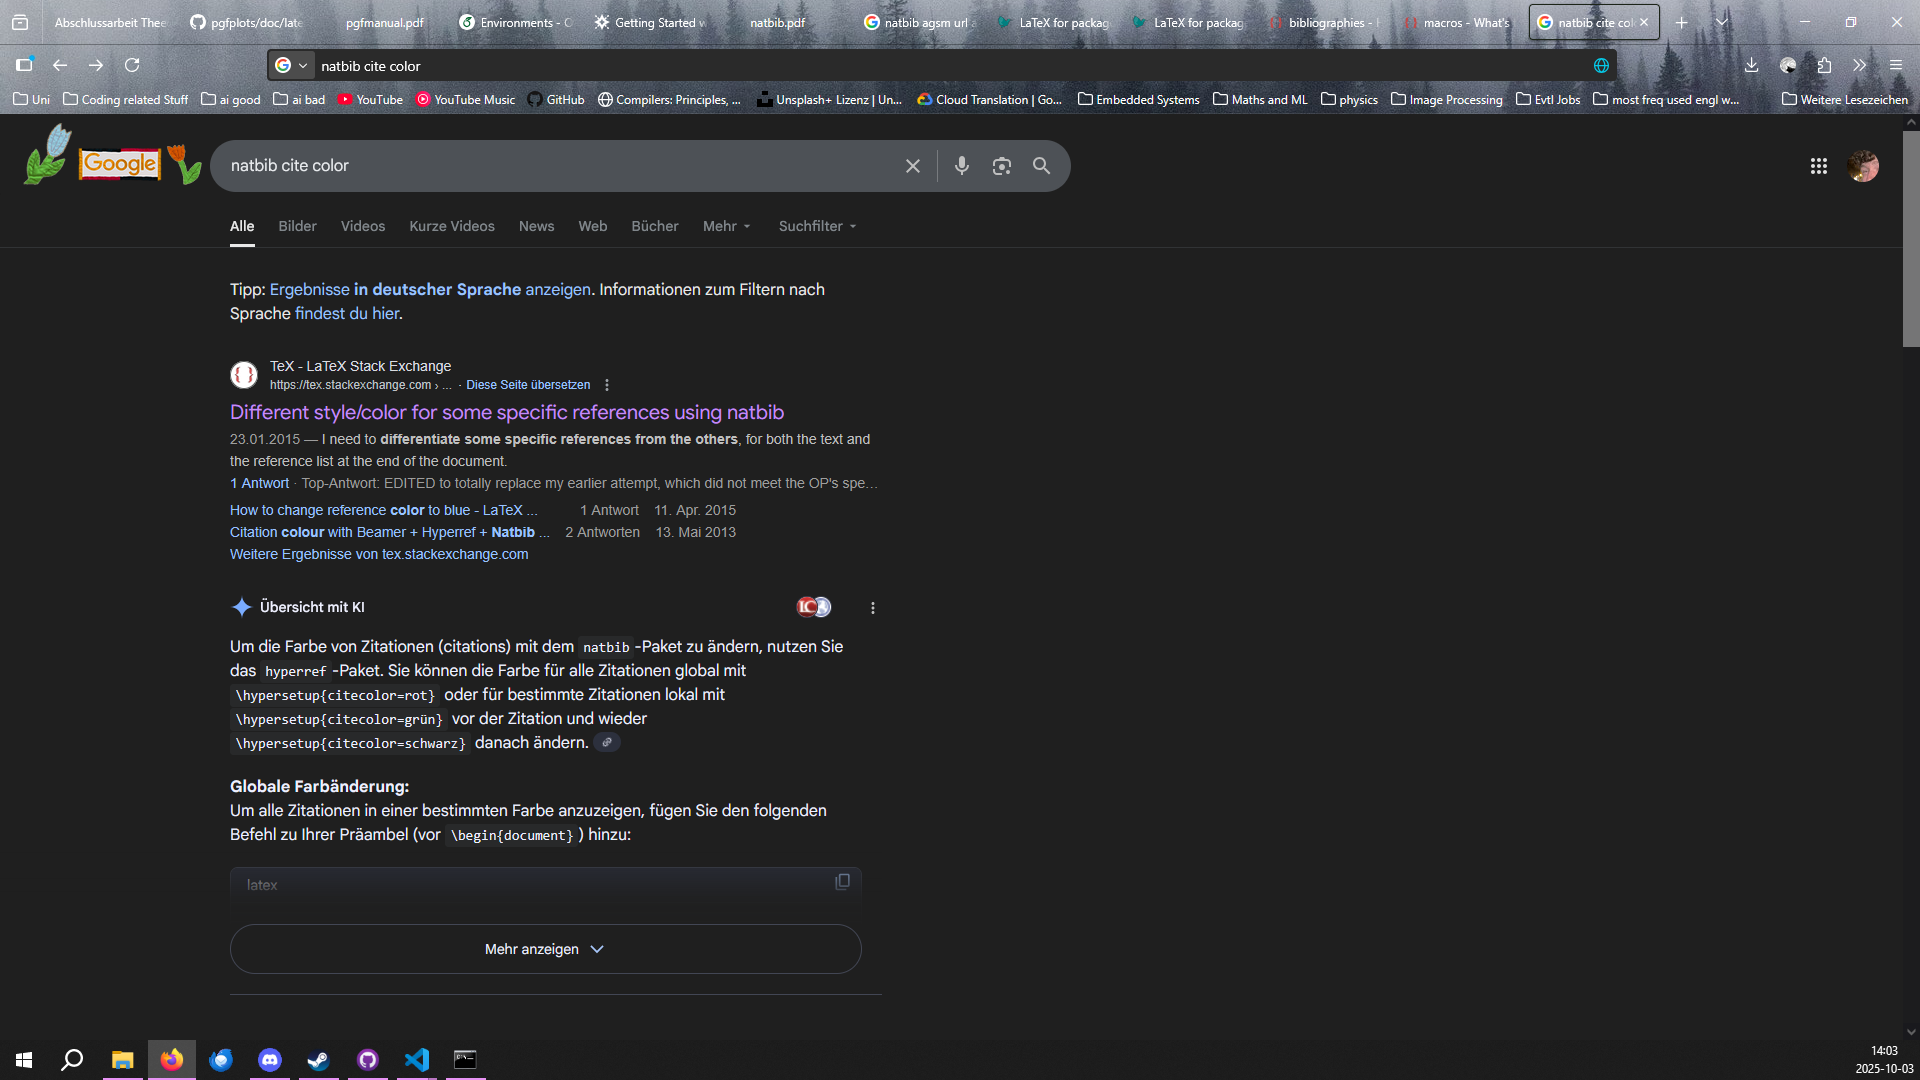
\includegraphics[width=\textwidth]{pictures/motivation.PNG}\label{fig:googlemakesmistakes}
\end{figure}
\end{document}